\question \textbf{Ford-Fulkerson}

\begin{parts}
\part  Use the Ford-Fulkerson algorithm to find a maximum flow in the network.

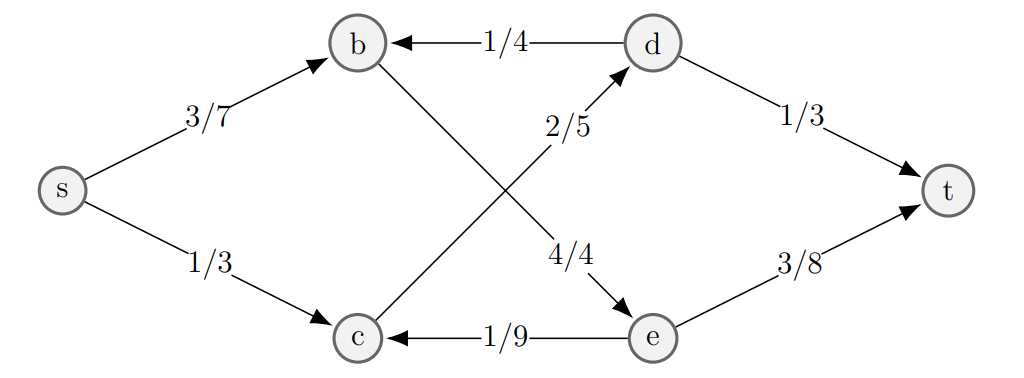
\includegraphics[width=0.6\linewidth]{task_2/task_2.png}

\begin{solution}
    
    
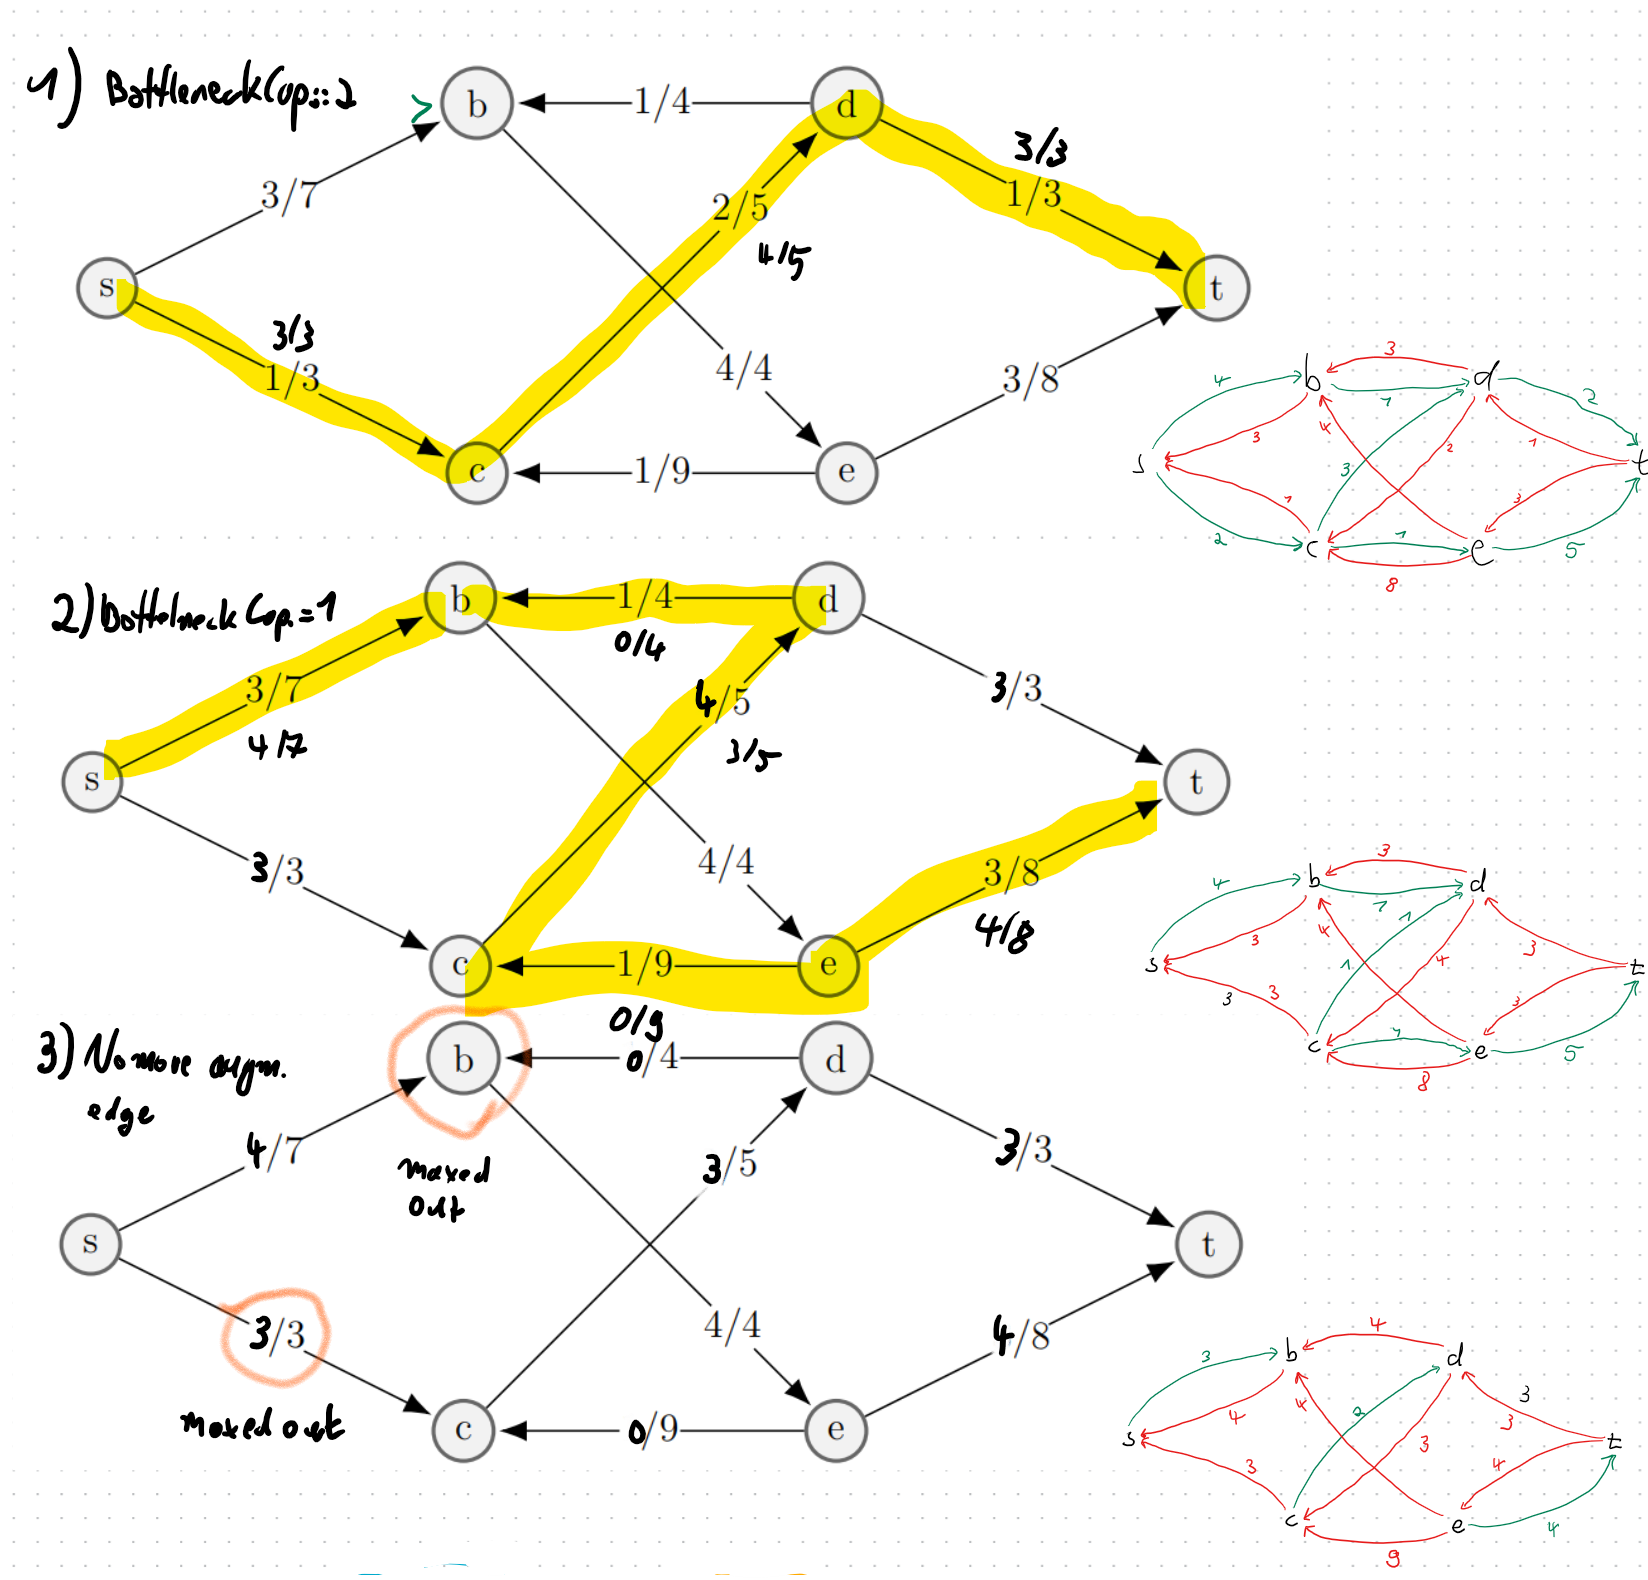
\includegraphics[width=0.9\linewidth]{task_2/sheet10_task2a_solution.png}
\end{solution}


\part Find a minimum cut proving the maximality of the flow.


\begin{solution}
    
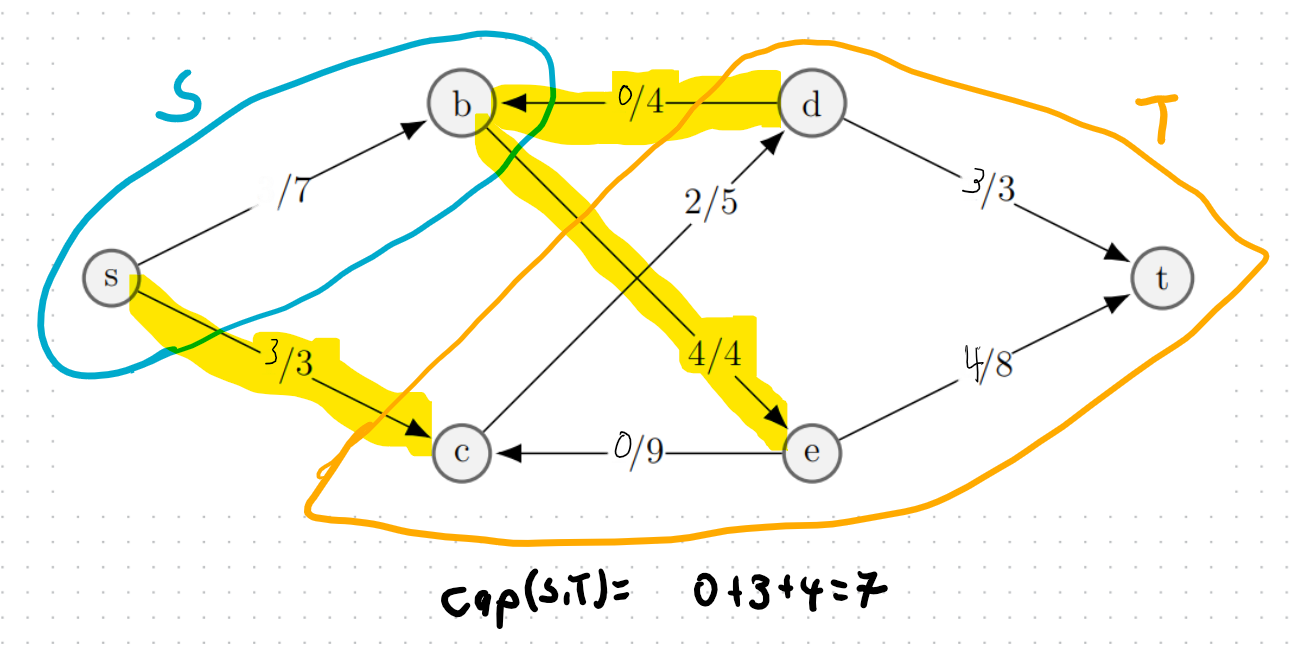
\includegraphics[width=0.6\linewidth]{task_2/sheet10_task2b_solution.png}
\end{solution}

\end{parts}


% For tasks without simply remove the \begin{parts}...\part...\end{parts} commands